% xelatex
\documentclass{article}

\usepackage[utf8]{inputenc}
\usepackage{fontspec}
\usepackage[margin=.75in]{geometry}

\usepackage{graphicx}
\graphicspath{ {./images/} }
\usepackage{ot-tableau}
\usepackage[backend=biber, style=authoryear-icomp]{biblatex}
\usepackage{textgreek}
\usepackage{easylist}
\usepackage{hanging}
\usepackage{hyperref}
\usepackage{blindtext}
\usepackage{tipa}
\usepackage{cgloss4e}
\usepackage{gb4e}
\usepackage{qtree}
\usepackage{enumerate}
\usepackage{longtable}
\usepackage{textgreek}
\usepackage{amsmath,amssymb,latexsym}
\usepackage{wasysym}
\setlength{\parindent}{0cm}

\pagenumbering{gobble}

\title{Bio Final Review}
\author{Daniel Filipski and Christopher Milan}

\begin{document}

\maketitle

\section{General Information}

\subsection{Where and when}

Friday, June 1st, 8:30 a.m. in the gym

\subsection{Topics}

Chapters 3-5 and 14-21

\subsection{Format}

Similar style to mid year exam, short answer and free-response. Free-response questions will require you to make 
connections between units.

\section{Genetics}

\subsection{Sex-linked genes}

These are genes located on the sex chromosomes.
They will show different phenotype frequencies based on gender.

\begin{exe}
\ex Gene A is on the X chromosome.
A is the wild type, and \textalpha \ is the diseased type.\\
X\textsuperscript{A}X\textsuperscript{\textalpha} $\times$ X\textsuperscript{A}Y:\\

\begin{tabular}{l | l}
X\textsuperscript{A}Y & X\textsuperscript{\textalpha}Y\\
X\textsuperscript{A}X\textsuperscript{A}  & X\textsuperscript{\textalpha}X\textsuperscript{A}\\

\end{tabular}
\end{exe}

\subsection{Pedigrees}
\Circle \ = Unaffected Female\\
\CIRCLE \ = Affected Female\\
$\square$ = Unaffected Male\\
$\blacksquare$ = Affected Male\\
\\
Connecting lines on pedigrees work just as they do on family trees.
Relatively simple logic can be used to determine the genotypes of each member of the pedigree; however, some can be more difficult than others.
My general method is to use the ``method of staring'' in the words of Mr. Letarte.

\subsection{Genetic Disorders -- Sickle Cell, Cystic Fibrosis, Huntington's}
\textbf{Sickle Cell}
\begin{itemize}
\item Red blood cells contain hemoglobin, which bind O\textsubscript{2}
\item Hemoglobin is made up of two \textalpha -goblin and two \textbeta -globin polypeptides
\item Mutation in \textbeta -globin makes it slightly less soluble
\item When O\textsubscript{2} is low, hemoglobin without O\textsubscript{2} will start to
clump and form long fibers that will change the shape of the red blood cell, which will then get stuck in capillaries
\item If one is a heterozygote of this disease, they have an advantage against milleria
\item Sickle Cell disease is recessive, because its effects are not great enough with only some of the \textbeta -globin broken.
\end{itemize}

\textbf{Cystic Fibrosis}
\begin{itemize}
\item In frame three base pair deletion in gene for CFTR
\item CFTR is missing one amino acid (phenylalanine), which causes it to misfold and be
destroyed
\item CFTR is a channel in the epithelial cell membranes for Cl\textsuperscript{-}
\item Without CFTR, there is too much extracellular Cl\textsuperscript{-}, which makes the fluid outside the cell thicker
\item Mucus clogs lungs and serves as a growth substance for pseudomonas aerougenase
\item The allele for Cystic Fibrosis is recessive, as with one of the two CFTR, cells still have enough paths for Cl\textsuperscript{-}
\end{itemize}

\textbf{Huntington's Disease}
\begin{itemize}
\item Mutation is dominant, but the disease does not present itself until late 30's or early 40's
\item Huntingtin gene expressed in nerve cells. Its developmental role in adults is unclear
\item CAG (codes for glutamine)
\item Wild type 6-35 repeats
\item Diseased 36+ repeats
\item Diseased protein forms aggretes in neurons, which lead to cell death.
\end{itemize}

\subsection{Nondisjunction}

Nondisjunction Event -- Failure to separate chromosomes\\
This is more common in meiosis I. Trisomy 21 causes down syndrome.

\subsection{Recombinant DNA -- Restriction Enzymes, Ligase, Electrophoresis, GFP, PCR, Selectable Markers, Screens, Plasmids, Transformations}
Recombinant DNA -- Combination of two or more pieces of DNA to create an artificial construct.\\
\\
Building Pieces of DNA:
\begin{enumerate}
\item Synthesize from scratch
\item Cut and Paste
\begin{itemize}
\item Ligase is not specific and will join any two pieces of DNA.
\item Restriction enzymes originate from bacteria, where they served s a type of immune system.
\item Restriction System: methylase adds CH\textsubscript{3}
\item Restriction Enzyme cuts DNA if not regulated.
\end{itemize}
\end{enumerate}

Eco RI:
\begin{itemize}
\item Sticky ends of $GAATTC$ (a DNA reverse palindrome)
\item Eco RI cuts between the G and the A
\end{itemize}

Plasmid:
\begin{itemize}
\item Mini chromosome in bacteria
\item Must have an ori, a selectable marker
\item Plasmids can be shared between cells. They also can be picked up from the
environment, when they are there for whatever reason.
\item An example of plasmids which can be shared between cells is antibiotic resistance.
\end{itemize}

DNA Sequencing:
\begin{itemize}
\item Denature DNA into single strands
\item Add primer for only one strand
\item Provide DNA polymerase and the four nucleotides, with a small fraction of the nucleotides modified so that DNA polymerase cannot extend from them (remove 3 hydroxyl)
\end{itemize}

GFP -- Green Fluorescent Protein\\
\indent GFP is used to see where or when certain promoters are expressed and to tag proteins.\\

PCR -- Polymerase Chain Reaction\\
\begin{itemize}
\item Amplify a specific DNA Sequence
\item NEED: Template DNA, Primers, DNA Polymerase, nucleotides (all four)
\item Three steps
\begin{enumerate}
\item Denature -- Use heat to separate the helix
\item Anneal -- Lower the tempurature, so the primers can bind
\item Extension -- Polymerase extends from the primers
\item Repeat steps 1 - 3 around 30 or 40 times
\end{enumerate}

\end{itemize}


\subsection{Selective Breeding -- Hybridization vs Inbreeding}

Selective breeding -- only allowing parents with certain characteristics to breed.\\
Hybridization:
\begin{itemize}
\item Crossing two organisms (typically plants) to get the best traits from both in a hybrid
\item Can be different species.
\end{itemize}\
Inbreeding:
\begin{itemize}
\item Continued breeding of individuals with similar characteristics
\item Dramatically decreases genetic variation
\item Increases prominence of some traits
\end{itemize}

\section{Evolution} %This section will be done tonight.

\subsection{Darwin's Observations and Background Knowledge}
Darwin made three key observations:
\begin{enumerate}
\item Species vary globally.
\item Species vary locally.
\item Species vary over time.
\end{enumerate}
More specifcally, there are the same types of animals in the same enviroments across the globe (ie. emu, ostritch, and reah)
Also Darwin made the observation about the finches and stuff.
That leads nicely into the next section, so read that.

\subsection{Evolutionary Theory -- Adaptations, Fitness, Natural Selection, etc.}
%Natural Selection -- Members of a population must compete for resources (food, water, space, etc.),
%and only the most fit can survive.\\
Natural Selection -- the process by which individuals with greater fitness survive and leave behind more offspring.
This occurs whenever more individuals are born than can survive, there is heritable variation, and that variation leads to varying levels of fitness.\\
\\
Adaptation -- any heritable characteristic that increase an organism's chance to survive and reproduce.\\
\\
Fitness -- how well an organism can survive in its enviroment.

\subsection{Evidence for Evolution}
\begin{itemize}
\item Fossil Record -- evidence for common decent
\item Carbon Dating -- the Earth is around 4.6 billion years old
\item Homologous Structures -- Structures that are shared by related species and were inheirited from a common ancestor
\item Cestigial Structures -- Structures that are inheirited from common ancestors and no longer used
\item Analogous Structures -- Structures that share a common function but not a common structure.
\item Embyology (The Study of Embryo Developement) -- The early stages of developement of embryos look very similar for vertibrates
\item Genetic Code -- all living things use DNA as the genetic material, transcribe RNA from DNA, and translate proteins from RNA. Triplet code is nearly universal.
\item Homologous Proteins and RNA -- Proteins and RNA that share similar structure and function.
\end{itemize}

\subsection{Population Genetics -- Hardy-Weinberg Equation and Conditions that disrupt equilibrium, selection on polygenic traits}
Hardy-Weinberg Principle -- allele frequencies remain constant unless one or more factors cause them to change.\\
\\
Single gene trait with two alleles. Define $p$ and $q$ as the allele frequencies, with $p$ as the dominant allele and $q$ as the recessive allele.\\
\\
Hardy-Weinberg Equation: $p^{2}+2pq+q^{2}=1$ or $p+q=1$\\

\begin{tabular}{| c | c |}
\hline
$p^{2}$ & $qp$\\
\hline
$pq$ & $q^{2}$\\
\hline
\end{tabular}
\\
\\
\\
Example: Mouse Populations\\
\begin{tabular}{|p{10cm}}
50\% AA [BLACKMOUSE] 50 Mice\\
40\% Aa [BLACKMOUSE] 40 Mice\\
10\% aa [WHITEMOUSE] 10 Mice\\
$P(AA)=p^{2}\Rightarrow f(A)^{2}=0.49$\\
$P(Aa)=2pq=0.42$\\
$P(a)=q^{2}$\\
\end{tabular}

Disruptions of Equilibrium:\\
\begin{enumerate}
\item Natural Selection
\item Mutations
\item Migration (Immigration and Emmigration)
\item Nonrandom Mating (Sexual Selection)
\item Small Population
\begin{itemize}
\item Bottle Neck Effect
\item Founder Effect
\end{itemize}
\end{enumerate}
Polygenic selection on next page.

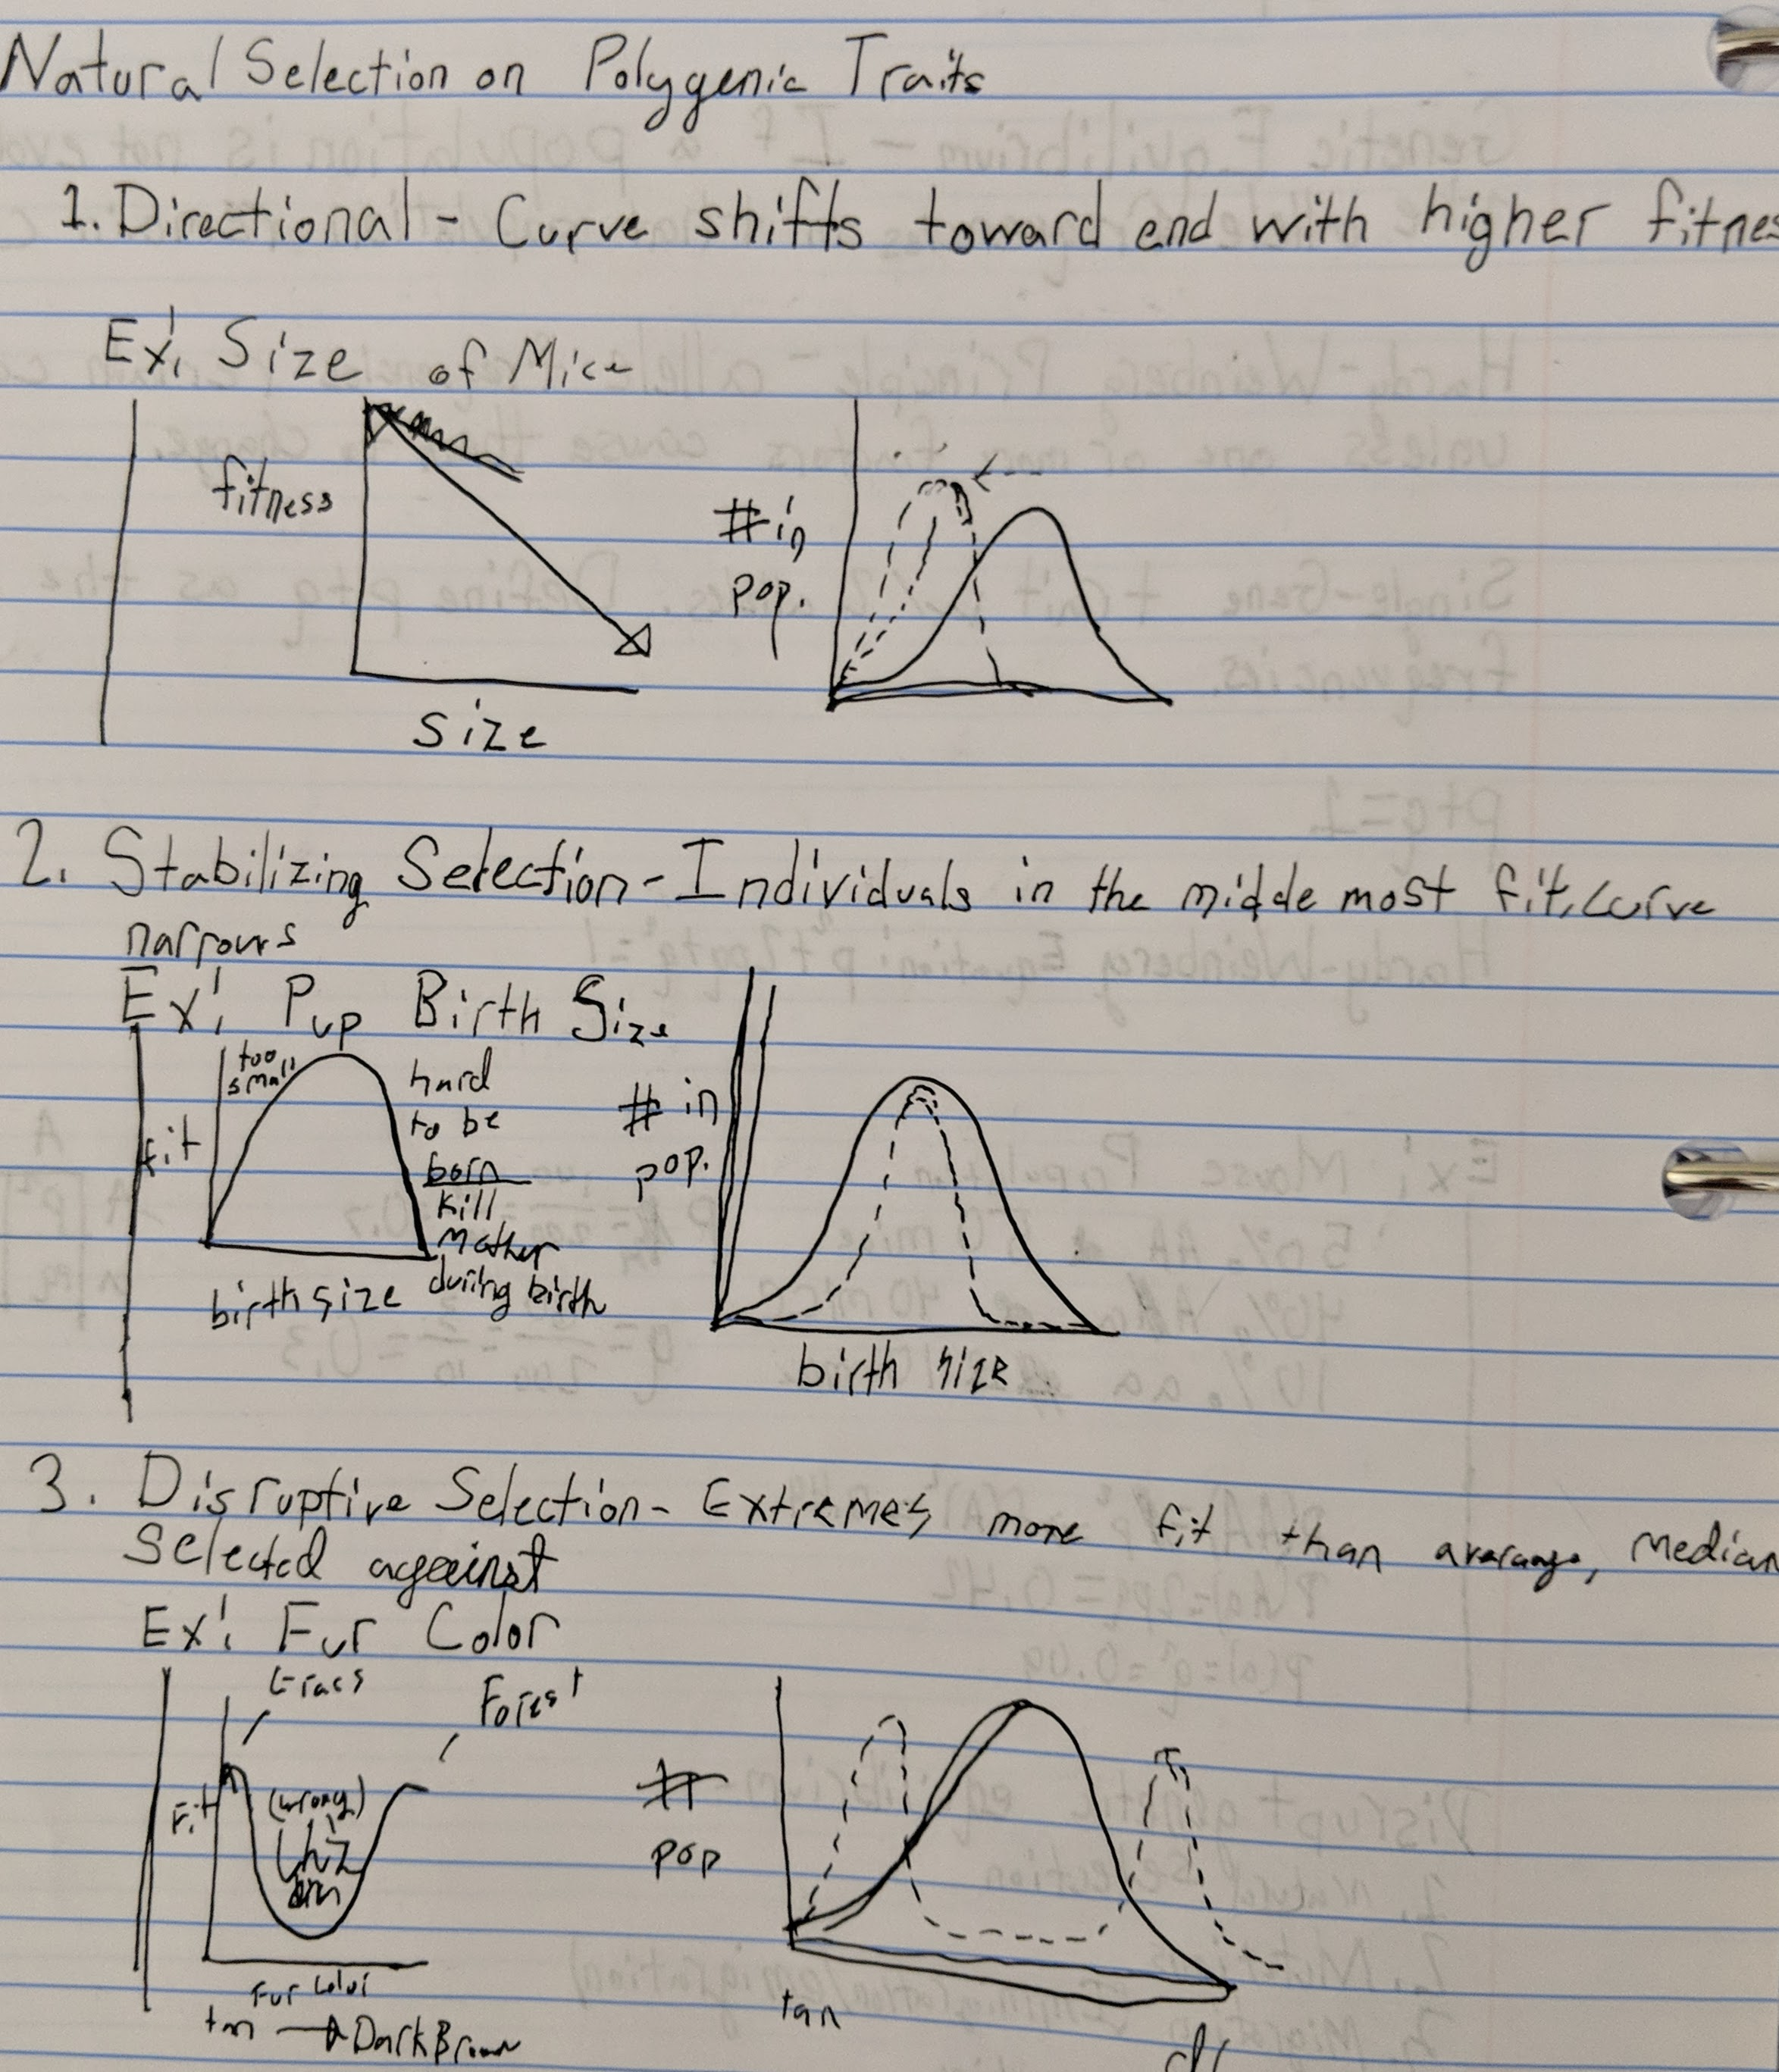
\includegraphics[scale=0.2]{multigenegraphs}
\subsection{Speciation}
Species -- Population that breeds together\\
\\
Reproductive Isolation -- Two populations can no longer interbreed and mat evolve into two different species\\
Types of Isolation:
\begin{enumerate}
\item Geographic Isolation -- Population physically separated
\item Behaivioral Isolation -- Differences in courtship rituals or methods
\item Temporal Isolation -- Two populations do not mate at the same time
\end{enumerate}

\subsection{Molecular Clocks}
Molecular Clock -- Use mutation rates in DNA to estimate when two species diverged from a common ancestor
\begin{itemize}
\item Most mutations are neutral, which means they accumalte over time
\item Some genes tolerate mutations better than others
\item The greater the number of differences in the DNA sequences of two species, the more time has elapsed since sharing a common ancestor.
\end{itemize}

\subsection{Binomial Nomenclature and Linnaean Classification}
Systematics -- Science of naming and grouping organisms into taxa that have biological meaning.\\
\\
Binomial Nomenclature -- two word science names\\
\\
Linaean Classification System:
\begin{itemize}
\item Domain
\item Kingdom
\item Phylum
\item Class
\item Order
\item Family
\item Genus
\item Species
\end{itemize}
These can be remembered via the snazzy acronym \textbf{K}aty \textbf{P}erry \textbf{C}laims \textbf{T}hat \textbf{O}rgasms \textbf{F}eel \textbf{G}ood \textbf{S}ometimes.\\
\\
\begin{tabular}{| c | c |}
\hline
Domain & Kingdoms within\\
\hline
Bacteria & Eubacteria\\
\hline
Archaea & Archaea Bacteria\\
\hline
Eukarya & Protists, Fungi, Plants, Animals\\
\hline

\end{tabular}

\subsection{Cladograms}
Clade -- a group of species that includes a single common ancestor and all descendants of that ancestor, living or dead\\
\\
Monphyletic vs. Paraphyletic -- paraphyletic groups are missing a common ancestor or contain multiple common ancestors or are missing descendants
\\
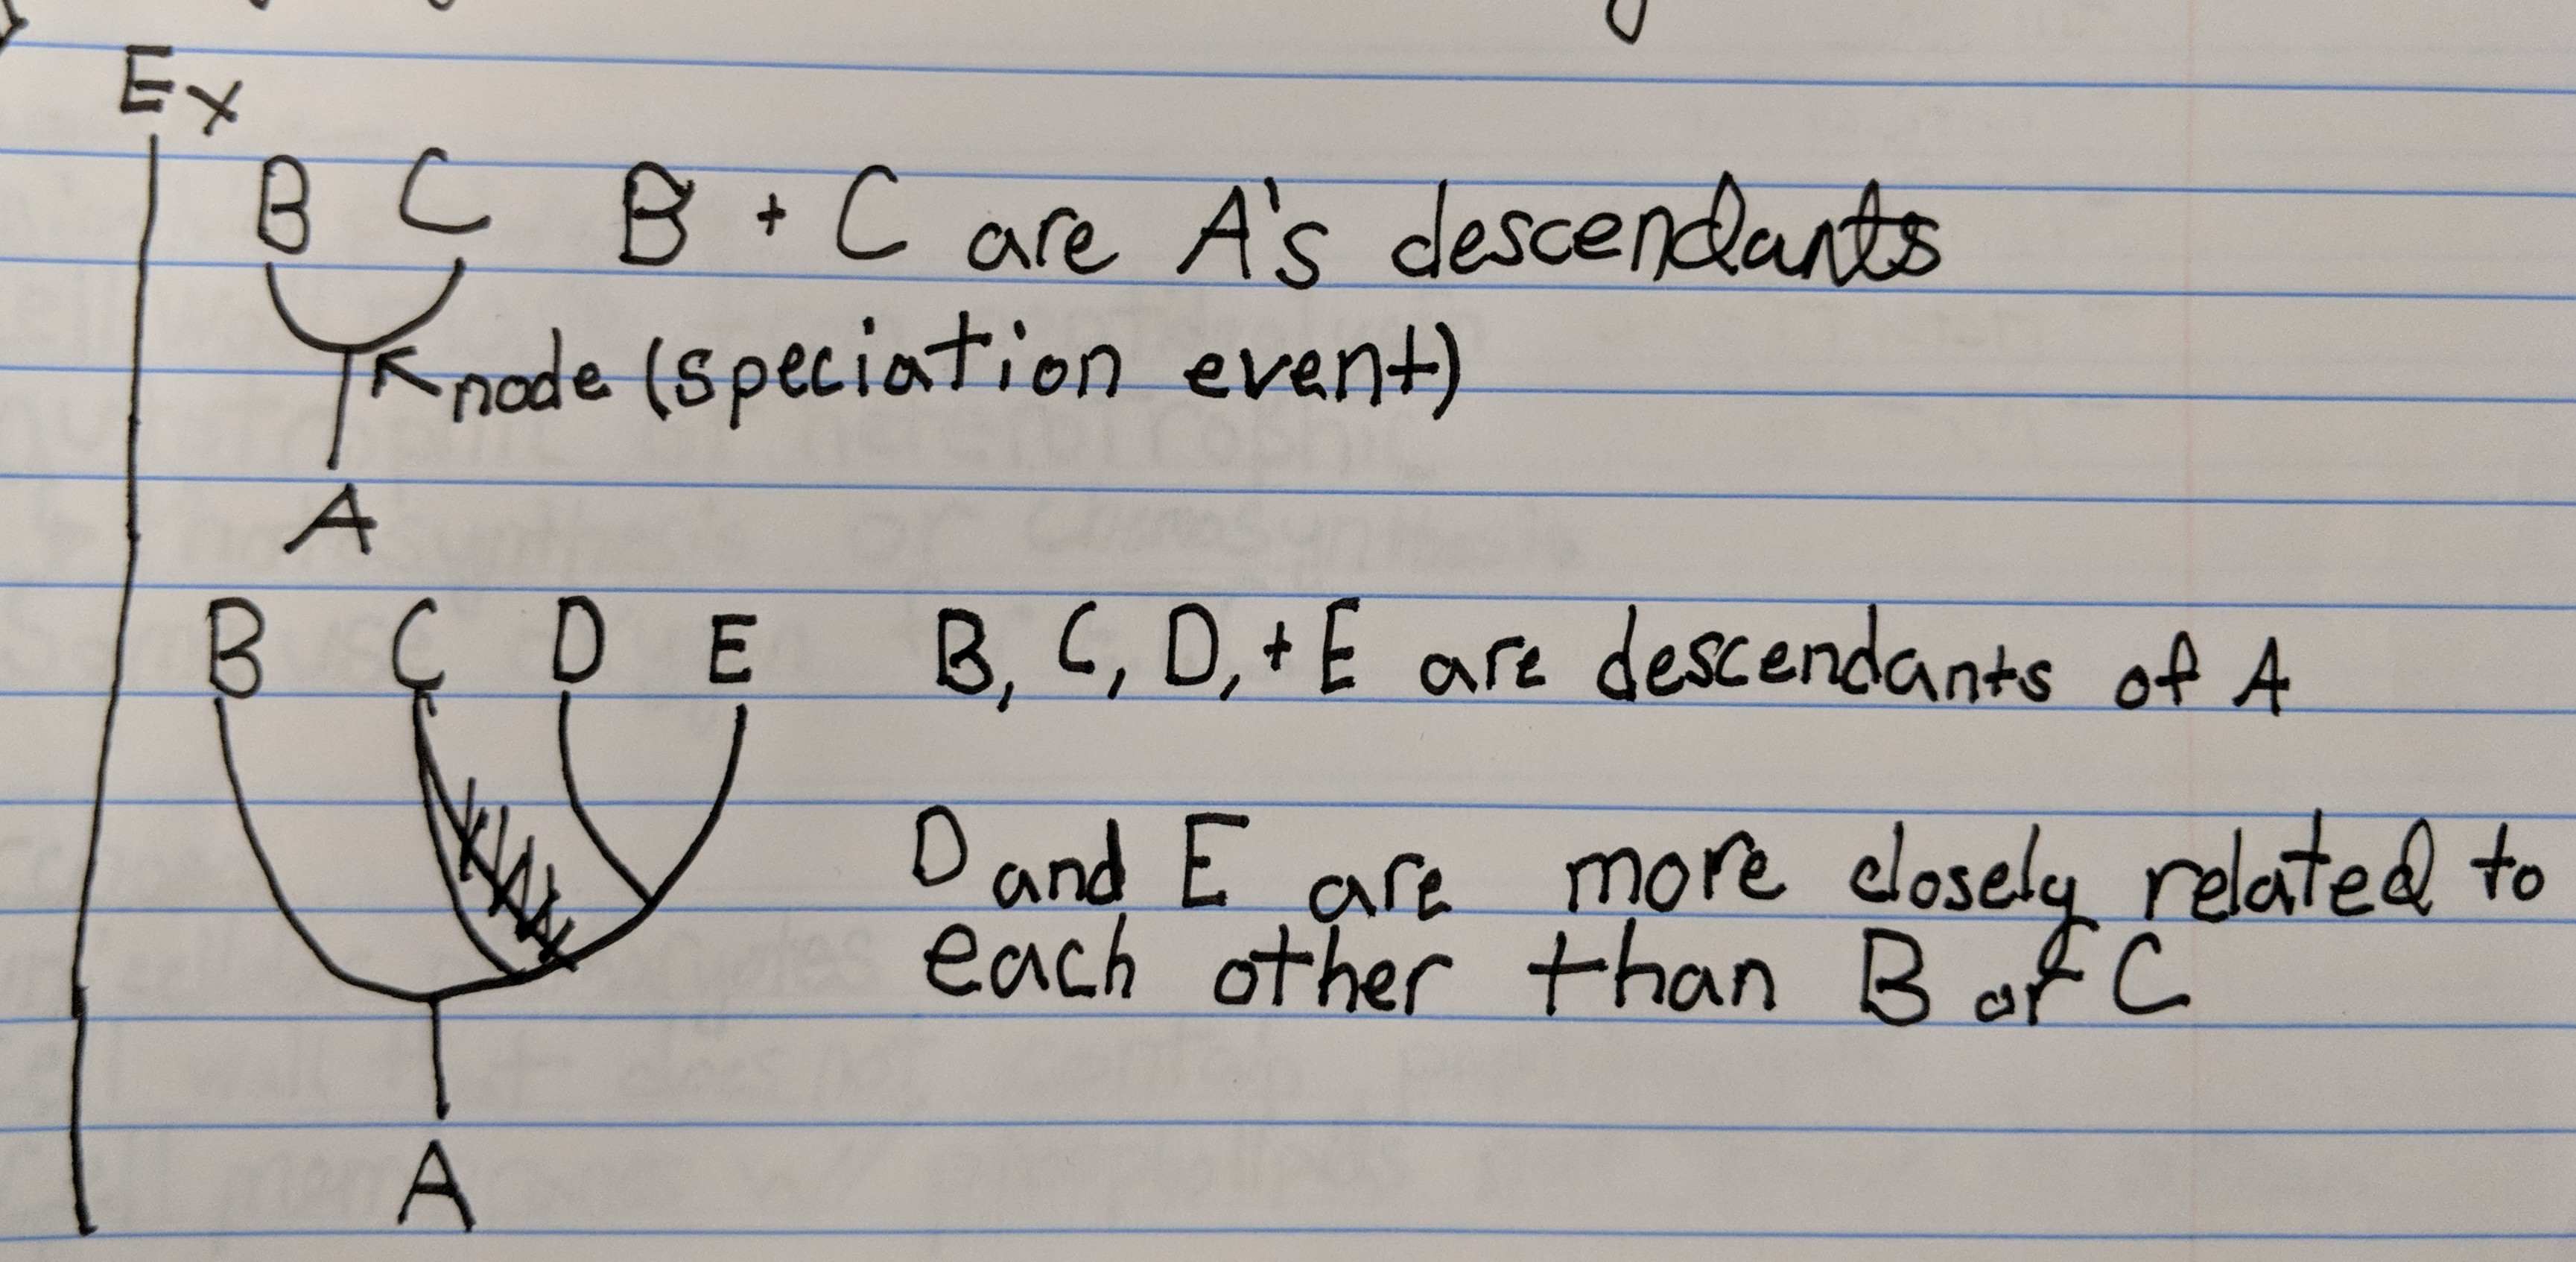
\includegraphics[scale=0.1]{cladogram}\\
\\
Buildings Cladograms:
\begin{itemize}
\item derived characteristic -- trait that arose in the most recent common ancestor of a lineage and was passed along to its descendants
\item parsimony (Occam's Razor) -- the simplest explanation is often correct.
\end{itemize}

\subsection{Domains and Kingdoms}

Bacteria:
\begin{itemize}
\item Unicellular Prokaryotes
\item Cell wall made from peptidoglycan
\item autotrophhic (photosynthesis or chemosynthesis) or heterotrophic
\item Some use oxygen for E.T.C.
\end{itemize}

Archaea:
\begin{itemize}
\item Unicellular Prokaryotes
\item Cell wall that doesn't contain peptidoglycen
\item Cell membranes with phospholipids not found in other domains
\item Autotrophic (chemosynthesis) or heterotrophic
\item Killed by O_2
\end{itemize}

Protists
\begin{itemize}
\item Unincellular, Colonies and Multicellular (brown algae)
\item At least five clades -- one closely related to funi, another to plants, and another to animals
\item Some have cellulose cell walls
\item Autotrophic (photosynthesis) or Heterotrophic
\end{itemize}

Fungi:
\begin{itemize}
\item Most multicellular, some unicellular
\item Cell walls made from chitin
\item Heterotrophs (detritivores or decomposers)
\end{itemize}

Plants:
\begin{itemize}
\item Most multicellular, some unicellular (green algae)
\item Cell wall from cellulose
\item Autotrophs (photosynthesis) \item nonmotile \end{itemize} Animals: \begin{itemize} \item Multicellular \item No cell wall \item Heterotrophs \item Motile \end{itemize}

\subsection{Fossil Record}
\begin{itemize}
\item Most fossils preserved in sedimentary rock
\item Made when organism falls in water and is buried in sand, silt, or mud. Then the sedimentary rock process happens. Shell, bones, and teeth remain if buried slowly. Soft tissue only remains if buried quickly.
\item Dating Fossils:
\begin{itemize}
\item Relative dating -- use index fossils to establish a temporal sequence
\item Radiometric dating -- use radioactive isotopes (they decay to get to stability)
\begin{itemize}
\item Kinetics of Decay:
\item $t=time$, $\lambda =$ $rate$ $constant$, $N_t =number$ $of$ $nuclei$ $at$ $time$ $t$, $N=initial$ $number$ $of$ $nuclei$, $t_{1/2}=half$ $life$
\item $\log_{10} {N_t/N_o} = -\lambda t$
\item $t_{1/2}={0.693}/{\lambda}$
\end{itemize}
\end{itemize}
\end{itemize}

\subsection{Origins of Life including Endosymbiont Theory}
\begin{itemize}
\item All life came from one cell
\item Prokaryote endosytosed another prokaryote
\item Didn't break it down
\item Mitochondria first
\item Chloroplast
\begin{itemize}
\item Evidence:
\item Small circlular chromosome in Mitochondria and Chloroplasts
\item Double membrane surround those two
\item Custom ribosome
\item Reproduce separatly from the rest of the cell
\end{itemize}
\end{itemize}

\subsection{Karyotypes}

A genome is the full set of genetic material. Karyotypes show this full genome, including the full diploid set of
chromosomes. They are:
\begin{itemize}
\item Grouped in pairs
\item In order of decreasing size
\end{itemize}

Example Karyotype:\\
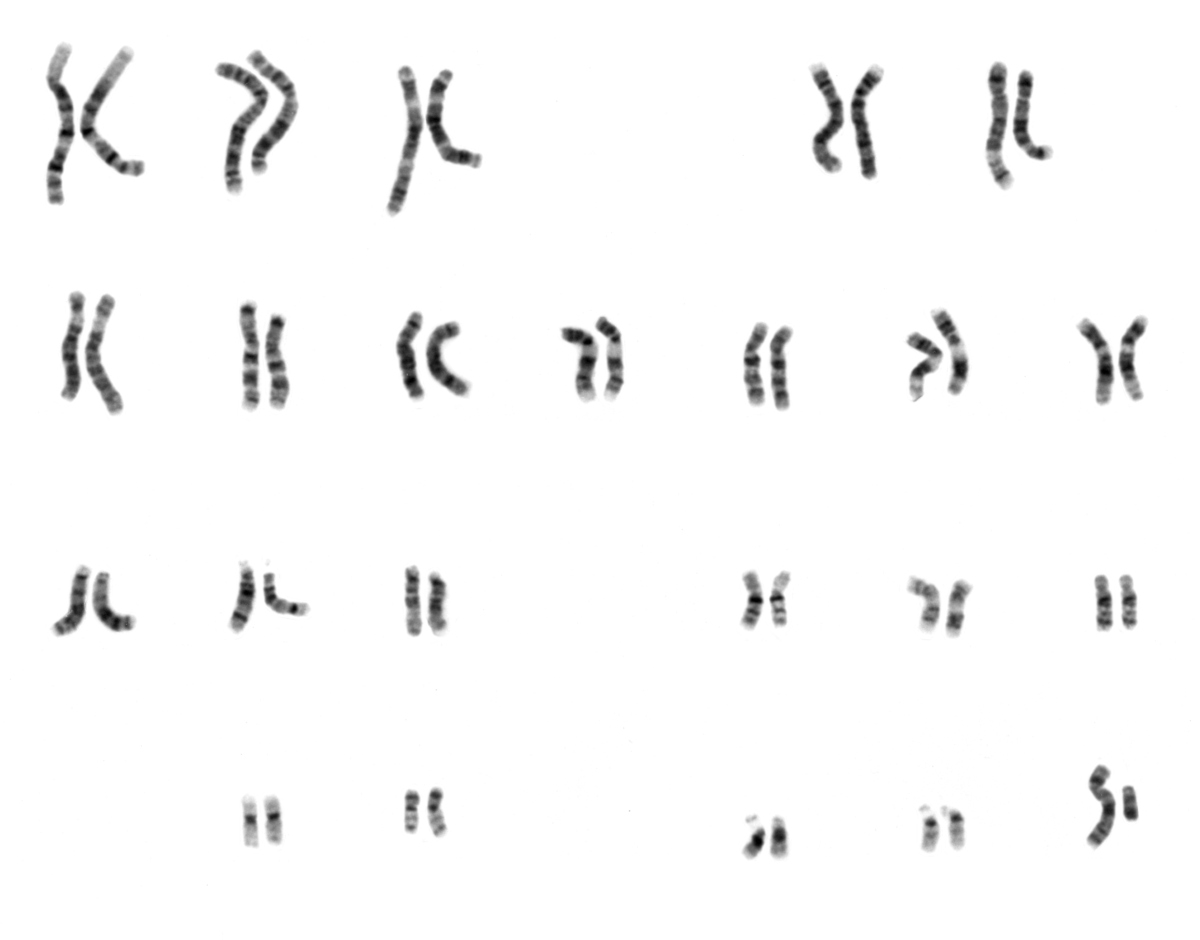
\includegraphics[width=0.5\textwidth]{karyotype}

Humans have 23 pairs of chromesomes, or 46 chromesomes in total.
\\
\\
Sex Chromosomes:
\begin{itemize}
\item Males - X and Y sex chromosomes
\item Females - X and X sex chromosomes
\end{itemize}
This ensures that zygotes will have an exactly 50/50 distrobution between male and female. There are approximately
1200 genes on the X chromosome and approximately 140 on the Y chromosome. The genes which are only found on the Y
chromosome specify male.
\\
\\
Autosomal Chromosomes:


\section{Ecology}

\subsection{Abiotic vs. Biotic Factors}
\begin{itemize}
\item Abiotic Factors -- physical factors in the enviroment
\item Biotic  Factors -- living factors in the enviroment
\end{itemize}

\subsection{Primary Producers vs. Consumers}
\begin{itemize}
\item Primary Producers -- Autotrophs. They make their own food using photo or chemosynthesis utilizing either solar or chemical energy to convert inorganic carbon to organic nutrients
\item Consumers -- Heterotrophs. Consume other orgnisms to get their nutrients. There are multiple levels (ie. primary, secondary, tertiary, etc.), with fewer amounts of organisms per level.
\end{itemize}

\subsection{Food Webs}
\begin{itemize}
\item Food Webs -- Network of interacting food chains
\item Food Chains -- Series of steps in which energy travels
\end{itemize}

\subsection{Trophic Levels and Ecological Pyramids}
\begin{itemize}
\item Trophic levels -- Each level in a food chain
\begin{itemize}
\item Primary producers are the first trophic level
\item Trophic levels are then different levels of consumers
\item There are also detritivores, but they don't really have a specific place in an ecological pyramid.
\end{itemize}
\end{itemize}

Ecoligcal Pyramids:
\begin{itemize}
\item Ecological Pyramid -- Shows the relative amount of energy or mater in each trophic level
\begin{itemize}
\item Types of Ecological Pyramids:
\item Energy Pyramid -- Energy that enters the ecosystem used for biological purposes. Much Energy is lost s heat. ~10\% of previous level's energy
\item Biomass Pyramid -- Organic tissue within each trophic level
\item Numbers Pyramid -- Number of organisms in each trophic level
\end{itemize}
\item GPP vs. NPP
\begin{itemize}
\item GPP -- Energy converted to chemical energy of organic molecules (per unit home)%probably misread
\item NPP -- Biomass availible to the next trophic level
\item $NPP=GPP-R_a$
\end{itemize}
\end{itemize}

\subsection{Nutrient Cycles}
%Add images of these later

\subsection{Niches and Competition}
\begin{itemize}
\item Niche -- Range of physical and biological conditions in which a species lives and the way in which it reproduces
\item Competition -- Organisms try to use the same resources at the same time
\begin{itemize}
\item intraspecific -- same species
\item interspecific -- different species
\end{itemize}
\item Competitive Exclusion Principle -- Two species cannot share a niche. There can be overlap, but not exact sharing.
\end{itemize}

\subsection{Keystone Species}
\begin{itemize}
\item Keystone Species -- Species the entire ecosystem relies on. The entire ecosystem can collpase with major changes to this population\\
\begin{tabular}{| p{10cm}}
Examples:\\
Pacific Sea Otters are a keystone species,  because they eat sea urchins, which do not have many other predators and could take over the exosystem if allowed to run rampant.
\end{tabular}
\end{itemize}

\subsection{Symbiosis}
Types of Symbiosis:
\begin{itemize}
\item Mutualism -- Both Species involved benefit
\item Parasitism -- One species benefits at the expense of another
\item Commonualism -- One species benefits, and the other neither benefits nor is harmed
\end{itemize}

\subsection{Succession}
\begin{itemize}
\item Ecological Succession -- A series of changes in a community. These are often predicatable and are caused by a disaster.
\item Primary Succession -- succession in an area where entire community was destroyed
\begin{itemize}
\item Can be caused by volcanic eruption, glacial recession, etc.
\item Lichen -- mutualism between a fungus and an alga (plant or protitst)
\begin{itemize}
\item Fix Nitrogen and Carbon
\item Can grow anywhere
\item Breaks down rocks and produces soil
\end{itemize}
\item Some grasses can be pioneer species
\begin{itemize}
\item Smaller, more effecient
\item Grow from the base, not the tip
\end{itemize}
\end{itemize}
\item Secondary Succession -- Succesion that begins in an area where some but not all of the community was destroyed
\begin{itemize}
\item Soil survives. This means that surviving plants and new vegatation can grow right away
\item Faster than primary Succesion
\end{itemize}
\end{itemize}

\subsection{Biomes -- Land and Aquatic}
We don't have to remember these, as far as I know.
She will give us the information we need, if she asks about biomes.

\subsection{Populations -- Defining Characteristics, growth models, and limiting factors}
\begin{itemize}
\item Population -- A group of organisms of a single species that live in a given area
\item A Population can be described with these things:
\begin{enumerate}
\item Geographic Range
\item Density and Distribution
\begin{itemize}
\item random, uniform, or clumped
\end{itemize}
\item Demographics
\begin{itemize}
\item age cohorts
\item growth rate
\item number of male and female
\end{itemize}
\end{enumerate}

\item Population growth
\begin{itemize}
\item Birth
\item Death
\item Immigration
\item Emmigration
\end{itemize}
\end{itemize}

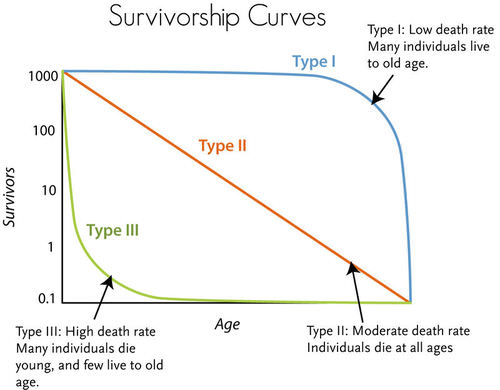
\includegraphics[scale=1.5]{ssc}

Exponential vs. Logistic Growth\\
Exponential growth happens in ideal conditions and is temporary.\\
Obviously, in exponential growth, the graph of population over time is that of an exponential function\\
${\triangle N}/{\triangle t}=B-D$, B is \# of Births, D is \# of Deaths\\
$B=bN$ $\leftarrow$ Average Birthrate\\
$D=dN$ $\leftarrow$ Average Deathrate\\
\includegraphics[scale=0.5]{log}\\
The population is constant once it reaches the carrying capacity.\\
${\triangle N}/{\triangle t}=rN(\frac{K-N}{K})$\\
This equation does not need to be memorized

Limiting Factors to Population Growth:
\begin{itemize}
\item Density Independent Factors
\begin{itemize}
\item Natural Disasters and Unusual Weather
\end{itemize}
\item Density Dependent Factors
\begin{itemize}
\item Competition (limited resources shared within a population)
\item Predation and Herbivory (Populations Cycle up and Down. May or may not be offset)
\item Parasites and disease ($\uparrow$ transmission of diseases with $\uparrow$ population)
\item Stress and Intrinsic Factors
\begin{itemize}
\item Behaivoral and Bacterial
\item Aggression rises with overpopulation
\item Neglect, kill, and or eat offspring
\item Delat sexual maturation, suppres immune system via hormonal changes
\end{itemize}
\item Waste Products
\end{itemize}
\end{itemize}

\subsection{Human Population Growth}
Growth Rate:
\begin{itemize}
\item Slow growth rate until around 650 (around 500mil people)
\item Period of exponential growth and birthrate remain high death rate dropped
\item Growth Rate peaked in early 1960s and has been descreasing
\end{itemize}

Demographic Transition:
\begin{itemize}
\item Movement from high birth and death rate to low birth and death rate
\item Tends to accompany industrialization and increase of living conditions
\item First High Birth and Death, Then High Birth and Low Death, Then Low Birth and Death
\end{itemize}
.\\

\begin{itemize}
\item Age structure -- relative number of individuals of each age in a population
\item Histograph -- depicts counts
\end{itemize}

Growth Predictions:
\begin{itemize}
\item Rapid growth -- young population smaller \% through age categories
\item Slow Growth -- around same \% until old age
\item No Growth -- Old Population
\end{itemize}

\end{document}
